\section{Diseño de la suite de simulación}

\subsection{Marco general del simulador}

Para la construcción de la suite de simulación, se debe tener en cuenta tanto la dinámica orbital como la dinámica de actitud, para así tener conocimiento del posicionamiento y la velocidad del CubeSat a través del espacio, y de la actitud de este en su desplazamiento alrededor de la Tierra. Para ello se debe considerar los siguientes elementos como base:

\begin{itemize}
	\item \textbf{\textit{Propagación orbital}}: En primera instancia, el simulador busca conocer el posicionamiento del satélite alrededor de la Tierra, por lo que es necesario el uso de un propagador orbital adecuado capaz de entregar información sobre el vector posición y velocidad del satélite respecto a la Tierra. Además, se debe considerar las perturbaciones correspondientes para la altura del satélite analizado, que en este caso se acotará a órbitas bajas, con el objetivo de hacer el movimiento traslacional del satélite realista según las condiciones espaciales presentes.
	
	\item \textbf{\textit{Modelos orbitales}}: Los modelos orbitales son necesarios para obtener la orientación del CubeSat. Con ello se obtendrán las representaciones necesarias de los sensores en el marco de referencia inercial.
	
	\item \textbf{\textit{Sensores}}: Para determinar la actitud del satélite, se seleccionan sensores capaces de entregar información relevante sobre la inercia del satélite, el comportamiento físico del ambiente espacial o estrellas circundantes. Es relevante tanto para la estimación inicial como para el conocimiento de la actitud a través del tiempo y se simularan según los modelos orbitales analizados, teniendo en cuenta una rotación del marco de referencia inercial al marco de referencia del cuerpo y el ruido en la lectura de los componentes utilizados.
	
	\item \textbf{\textit{Algoritmos de estimación de actitud}}: Estos son necesarios para trabajar los vectores entregados por los sensores y los modelos orbitales. Con estos se obtienen los cuaterniones que representan las rotaciones del satélite a través del tiempo. Se busca utilizar el \gls{EKF} para la estimación de los estados posteriores, además de una mitigación del ruido en la obtención de la orientación del satélite.
	
	\item \textbf{\textit{ Controladores y actuadores}}: Ya obtenidas la actitud del satélite a través del tiempo, se desea que el CubeSat apunte a una dirección en específico. Para ello se implementa el uso de un controlador capaz de realizar el control del satélite mediante la entrega del modelo dinámico y del actuador. Esto va de la mano con la selección del actuador a utilizar, para tener en cuenta las limitaciones de la acción de control al apuntar el satélite hacia la dirección deseada.
	
\end{itemize}

Teniendo en cuenta estos factores, la Figura~\ref{fig:bloq_gen} presenta un diagrama que resume la estructura de la suite de simulación, utilizada para obtener los resultados de los  MoP de apuntamiento y los SE envelopes correspondientes. En primer lugar, se obtiene el vector de estado $\vec{r}$ del CubeSat mediante el propagador orbital, seguido por el uso de modelos orbitales para calcular $\vec{V}_{ref}$, el vector en el sistema de referencia inercial. Simultáneamente, a través de la lectura de los sensores, se obtienen los vectores $\vec{V}_{obs}$ en el marco de referencia del cuerpo. Posteriormente, se realiza el cambio de sistema de referencia de $\vec{V}_{ref}$ a \gls{LVLH} (como se explicará en las secciones siguientes), utilizando ambos vectores para la estimación del cuaternión $q$. Finalmente, se ejecuta la acción de control mediante el controlador seleccionado, considerando la restricción del torque $\tau$ ejercido por el actuador. En las próximas secciones se detallará el diseño y selección de cada componente de la suite de simulación.

\begin{figure}[h]
	\centering    
	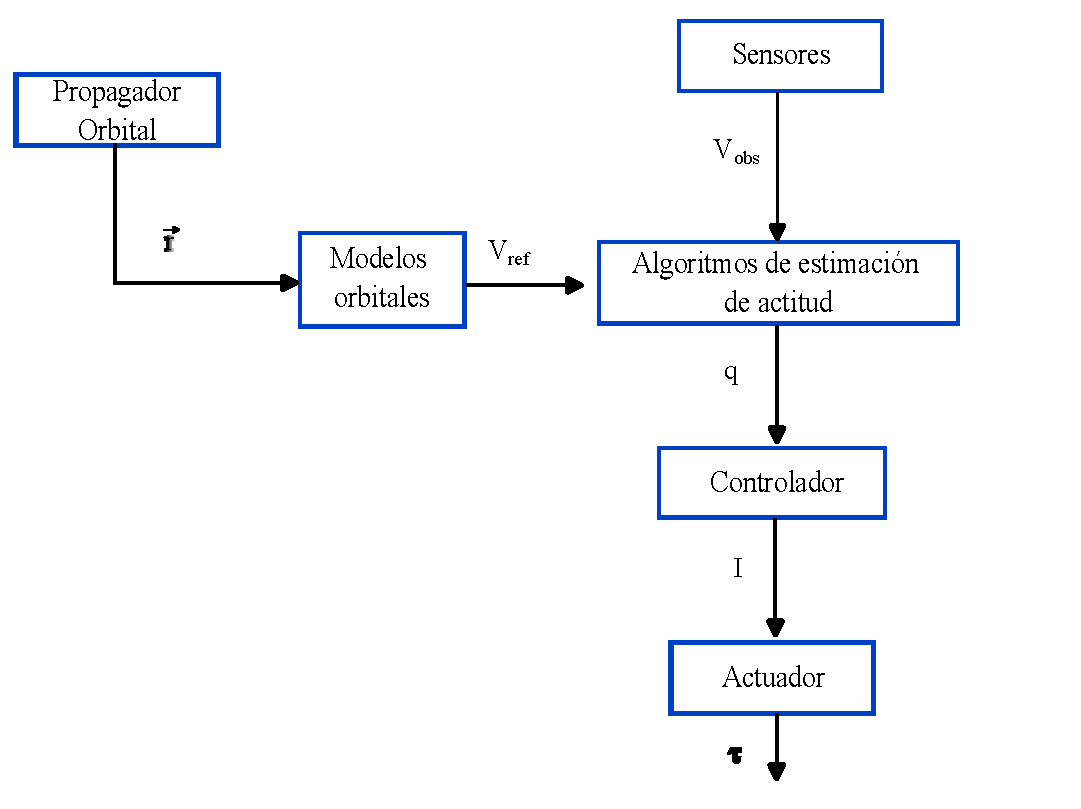
\includegraphics[width=0.65\textwidth]{bloques_generico.pdf}
	\caption{Esquema general de la base del simulador (Elaboración propia).}
	\label{fig:bloq_gen}
\end{figure}

\subsection{Propagador orbital}

Para la simulación de la dinámica orbital, se debe considerar la implementación de un propagador capaz de entregar la posición y velocidad del satélite respecto a la Tierra incluyendo las perturbaciones relevantes a baja altura. Para ello se proponen las siguientes opciones:

\textbf{\textit{\gls{SGP4} \cite{ref37}}}:Es un modelo matemático que se utiliza ampliamente para predecir la posición y velocidad de los satélites. Utiliza las ecuaciones de movimiento de dos cuerpos, que describen cómo un satélite se mueve bajo la influencia de la gravedad de la Tierra, y luego aplica una serie de perturbaciones para tener en cuenta factores como la forma no esférica de la Tierra, el arrastre atmosférico, la radiación solar y los efectos gravitacionales de la interacción con otros cuerpos como el Sol o la Luna. El SGP4 utiliza los \gls{TLE} como entrada, que es un formato estándar utilizado para describir la órbita de un satélite en dos líneas, en conjunto con la fecha de inicio y el tiempo de propagación, para después aplicar una serie de ecuaciones y algoritmos que calculan los elementos orbitales futuros del satélite en función del tiempo.

\textbf{\textit{FreeFlyer \cite{ref38}}}:Es un programa de simulación espacial diseñado para visualizar y modelar varios escenarios, incluyendo, pero no limitándose a la propagación y maniobras de naves espaciales, análisis de cobertura y contacto, análisis interplanetario y la generación de diversos recursos visuales. Es capaz de propagar el movimiento del satélite a través del tiempo e incluir perturbaciones como $J_2$, arrastre atmosférico, efecto multi-cuerpo y radiación solar.

\textbf{\textit{\gls{STK} \cite{ref34}}}: Es una plataforma ampliamente utilizada en el ámbito tanto aeronáutico como espacial. El STK es un simulador de Ansys utilizado para el diseño, planificación y simulación de misiones. Una de sus herramientas es la propagación del satélite a través del tiempo con una interfaz gráfica, incluyendo todas las perturbaciones presentes en el espacio.

Se descartan las opciones de los softwares FreeFlyer y STK debido a su alto costo monetario para la implementación del simulador solo para su uso en la dinámica orbital. Por lo tanto, se elige el SGP4 no solo por ser una opción gratuita, sino porque es fácil de implementar a cualquier satélite que se conozca su TLE. Esta entrega el movimiento traslacional del satélite a través del tiempo considerando las perturbaciones más importantes a bajas alturas.

Para analizar el funcionamiento del propagador, se utilizó como ejemplo un TLE del SUCHAI-3 obtenido de CelesTrak y se propagó durante un día tomando como fecha de inicio 1 de noviembre del 2023 a las 12 del mediodía. Se observa en la Figura~\ref{fig:pos} y ~\ref{fig:vel} la posición y la velocidad respecto al marco de referencia ECI obtenido en Python a través de la librería SGP4.

\begin{figure*}[h]
	\centering
	\begin{subfigure}[t]{0.68\textwidth}
		\centering{%
			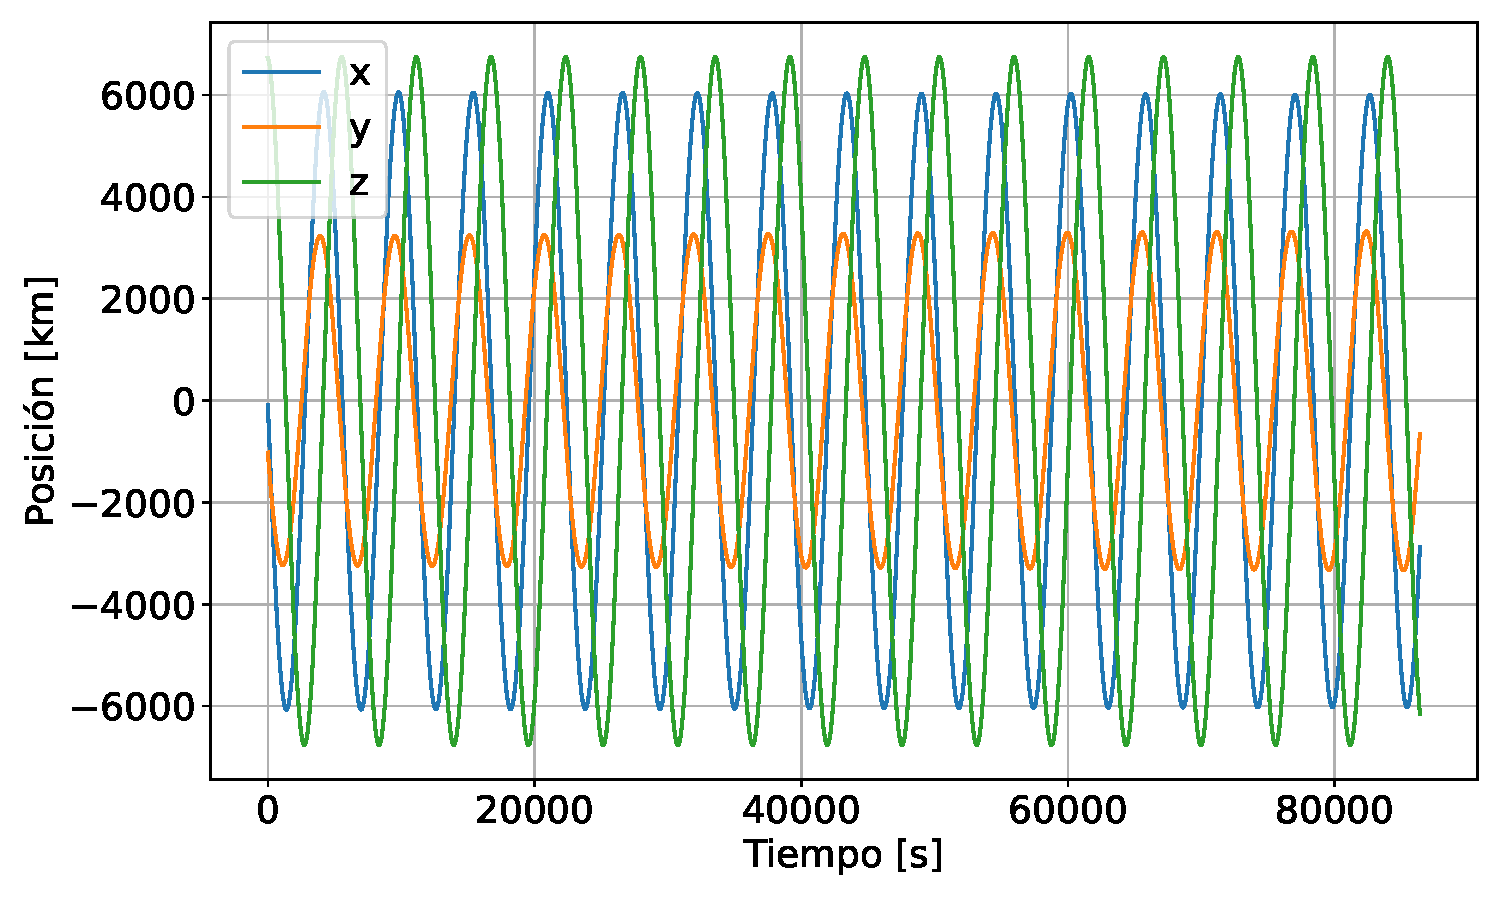
\includegraphics[width=\textwidth]{pos.pdf}
		}%
		\subcaption{Posición del satélite.\label{fig:pos}}
	\end{subfigure}
	\begin{subfigure}[t]{0.68\textwidth}
		\centering{%
			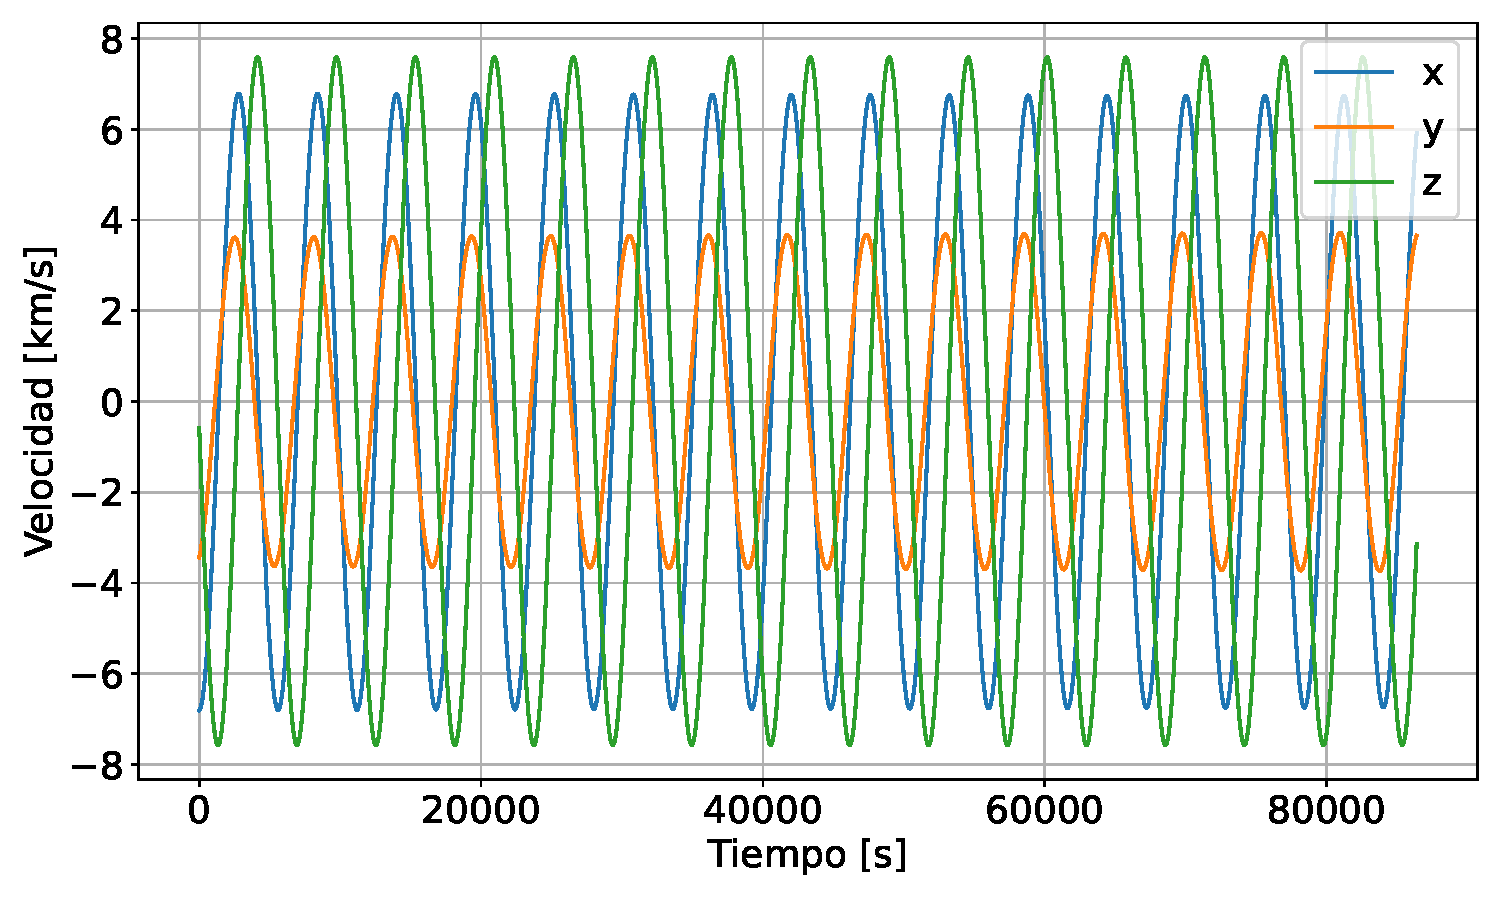
\includegraphics[width=\textwidth]{vel.pdf}
		}%
		\subcaption{Velocidad del satélite.\label{fig:vel}}
	\end{subfigure}
	\caption{Propagación del SUCHAI-3 durante un día con fecha de inicio 01/11/23.}\label{fig:pos-vel}
\end{figure*}


\subsection{Modelos orbitales y sistemas de referencia}

Para la obtención de la actitud del satélite se requieren conocer dos vectores respecto al marco de referencia Local Vertical Local Horizontal (LVLH) o también llamado orbital.  Para ello se conocerán en primera instancia los modelos del sol y del campo geomagnético terrestre para la obtención de los vectores en el marco de referencia inercial (ECI), para luego rotarlos al sistema LVLH. Posteriormente se obtendrán los vectores de observación, que se generan en base a los modelos mencionados aplicando otra rotación desde orbital al cuerpo, que representan los vectores medidos por los sensores.

\subsubsection{Vector sol}

El modelo se basa principalmente en el movimiento del sol respecto al sistema de referencia ECI. Lo primero a tener en cuenta es la anomalía media del sol, la cual se calcula según muestra la Ecuación~\ref{eq:M_sun} y consiste en el ángulo medido desde el perigeo, que describe la posición del Sol en su trayectoria orbital y depende puramente del tiempo \cite{ref15}.

\begin{equation}
	M_{\text{sun}} = M_{\text{sunEpoch}} + n_{\text{sun}}JD_{2000} = 357.528^\circ +   0.9856003^\circ \cdot JD_{2000}
	\label{eq:M_sun}
\end{equation}

En la ecuación anterior, $M_{\text{sunEpoch}}$ es el valor conocido de la anomalía media del Sol para el 1 de enero de 2000 al mediodía en UTC y $n_{\text{sun}}$ es el movimiento medio del Sol, el cual también es un valor conocido. La anomalía media del Sol puede entonces calcularse para cualquier $JD_{2000}$, que se refiere a la fecha juliana respecto al año 2000. A partir de la anomalía media, se puede calcular la longitud de la eclíptica $\lambda_{\text{sun}}$ según la Ecuación~\ref{eq:lambda_sun}, que representa la posición del Sol en el plano orbital bidimensional en el marco ECI.

\begin{equation}
	\lambda_{\text{sun}} = 280.461^\circ + 0.9856474^\circ \cdot JD_{2000} + 1.915^\circ \sin(M_{\text{sun}}) + 0.020^\circ \sin(2 M_{\text{sun}})
	\label{eq:lambda_sun}
\end{equation}

Para determinar completamente la posición del Sol en el marco ECI, se requiere conocimiento de la inclinación de la órbita desde el plano orbital bidimensional. Este parámetro se llama oblicuidad del plano de la eclíptica y se define en la Ecuacion~\ref{eq:eps_sun}

\begin{equation}
	\epsilon = 23.4393^\circ + 0.0000004^\circ \cdot JD_{2000}
	\label{eq:eps_sun}
\end{equation}

La posición del Sol en el marco ECI ahora se puede calcular como un vector unitario con las componentes representadas en la Ecuación~\ref{eq:x_sun}, ~\ref{eq:y_sun} y ~\ref{eq:z_sun}.

\begin{equation}
	X_{\text{sun}} = \cos(\lambda_{\text{sun}})
	\label{eq:x_sun}
\end{equation}

\begin{equation}
	Y_{\text{sun}} = \cos(\epsilon) \sin(\lambda_{\text{sun}})
	\label{eq:y_sun}
\end{equation}

\begin{equation}
	Z_{\text{sun}} = \sin(\epsilon) \sin(\lambda_{\text{sun}})
	\label{eq:z_sun}
\end{equation}

Este modelo del vector sol se observa en la Figura~\ref{fig:ss}, en la cual se simula propagando por un año desde el 01 de noviembre del 2023, el cual en días julianos corresponde al día 2460250. Se observa en dicha gráfica un comportamiento oscilatorio, notándose un ciclo entero del movimiento del sol recién al término de la simulación.

\begin{figure}[h]
	\centering    
	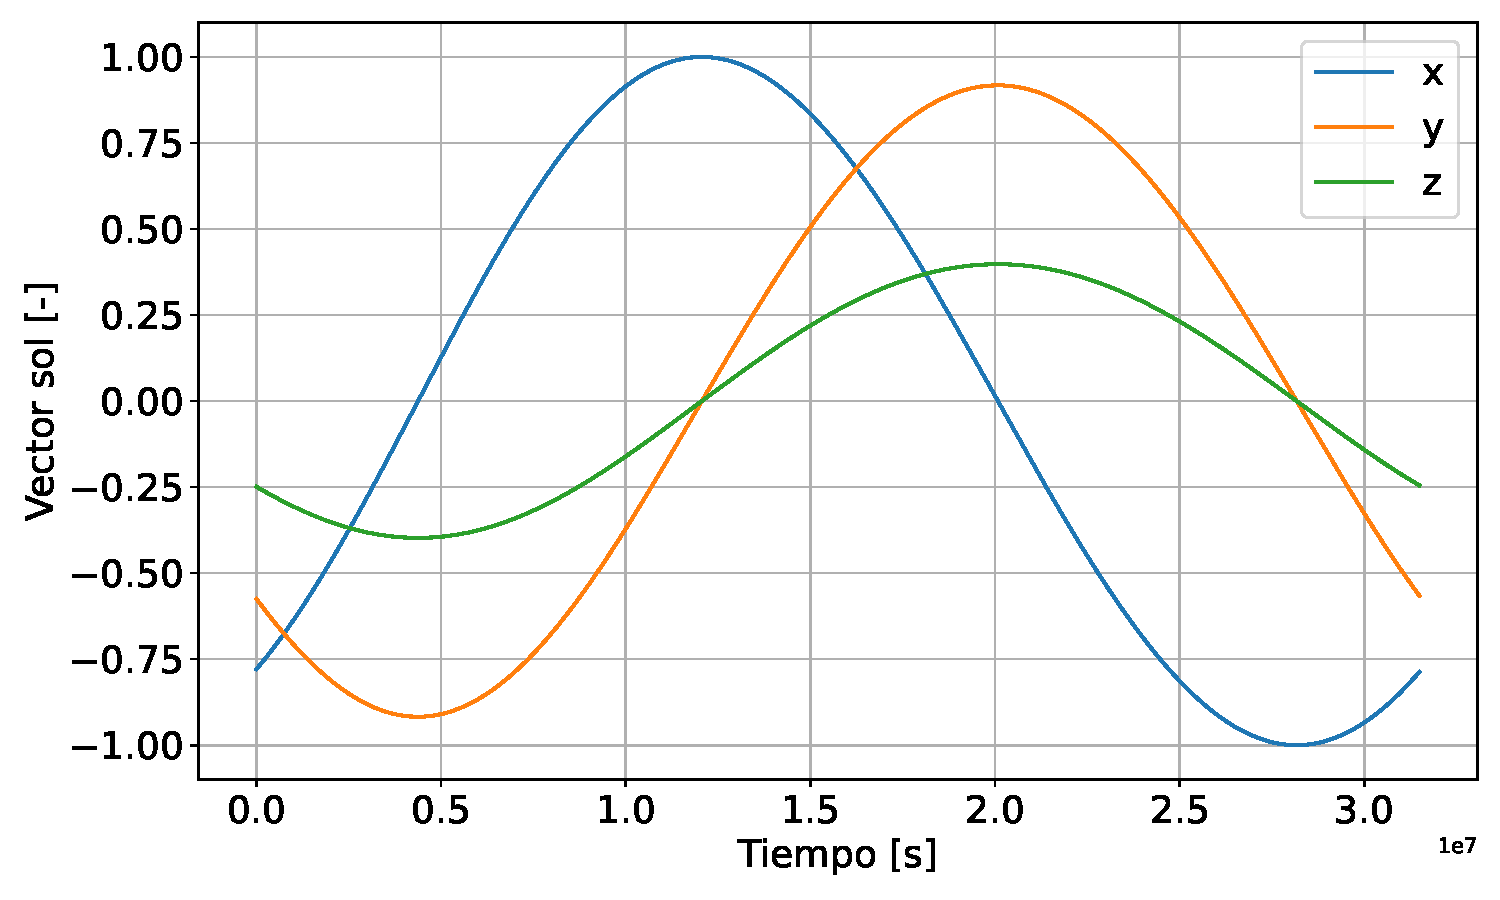
\includegraphics[width=0.65\textwidth]{ss.pdf}
	\caption{Vector sol en sus tres componentes simulados durante un año (Elaboración propia).}
	\label{fig:ss}
\end{figure}


\subsubsection{Fuerzas geomagnéticas de la Tierra}

Para el modelamiento de las fuerzas geomagnéticas de la tierra en distintas posiciones de la órbita de un satélite se requiere el uso del \gls{IGRF}. Este campo de referencia consiste en un conjunto de coeficientes armónicos esféricos que pueden introducirse en un modelo matemático, para así describir la porción a gran escala y variable en el tiempo del campo magnético interno de la Tierra entre las épocas 1900 d.C. y el presente. El IGRF utilizado para la realización del simulador es el de decima tercera generación y se ha derivado de observaciones registradas por satélites, observatorios terrestres y estudios magnéticos \cite{ref39}.

El IGRF describe el principal \gls{B} que es producido por fuentes internas, principalmente dentro del núcleo de la Tierra. El IGRF es válido dentro y alrededor de la superficie de la Tierra, donde el campo geomagnético principal puede describirse como el gradiente de un potencial escalar, $B = -\nabla V$, y la función potencial $V(r, \theta, \varphi, t)$ se representa en la Ecuación~\ref{eq:potencial} como una expansión en serie finita en términos de coeficientes armónicos esféricos, $g_n^m, h_n^m$, también conocidos como coeficientes de Gauss:

\begin{equation}
	V(r, \theta, \varphi, t) = a \sum_{n=1}^{N} \sum_{m=0}^{n} \left( \frac{a}{r} \right)^{n+1} 
	\left[ g_n^m(t) \cos(m \varphi) + h_n^m(t) \sin(m \varphi) \right] P_n^m(\cos(\theta))
	\label{eq:potencial}
\end{equation}

Aquí, $r, \theta, \varphi$ se refieren a coordenadas en un sistema de coordenadas esféricas geocéntricas o geodésicas, siendo $r$ la distancia radial desde el centro de la Tierra o la altura desde su superficie dependiendo de si son geocéntricas o geodésicas respectivamente, y $\theta, \varphi$ son la co-latitud y longitud geocéntricas respectivamente. 

Las $P_n^m (\cos(\theta))$ son funciones de Legendre asociadas seminormalizadas de Schmidt de grado $n$ y orden $m$. El parámetro $N$ especifica el grado máximo de expansión armónica esférica y se eligió que fuera 10 hasta la época 1995 inclusive, después de lo cual aumenta a 13. Por otro lado, los coeficientes de Gauss cambian en el tiempo y se proporcionan en unidades de nanoTesla (nT) en IGRF-13 en intervalos de época de 5 años. La dependencia temporal de estos parámetros se modela como lineal por partes y viene dada por:

\begin{equation}
	g_n^m (t) = g_n^m (T_t) + (t - T_t) \dot{g}_n^m (T_t)
\end{equation}

\begin{equation}
	h_n^m (t) = h_n^m (T_t) + (t - T_t) \dot{h}_n^m (T_t)
\end{equation}

Donde $g_n^m (T_t)$, $h_n^m (T_t)$ son los coeficientes de Gauss en la época $T_t$, que precede inmediatamente al tiempo $t$. Las épocas del modelo en IGRF-13 se proporcionan en múltiplos exactos de 5 años comenzando en 1900 y terminando en 2020, de modo que $T_t < t < T_t+5$. Para $T_t < 2020$, los parámetros $\dot{g}_n^m (T_t)$, $\dot{h}_n^m (T_t)$ representan la aproximación lineal al cambio en los coeficientes de Gauss durante el intervalo de 5 años que abarca $[T_t, T_t+5]$. Pueden calcularse en unidades de nanoTesla por año (nT/año) como:

\begin{equation}
	\dot{g}_n^m (T_t) = \frac{1}{5} \left( g_n^m (T_t+5) - g_n^m (T_t) \right)
\end{equation}

\begin{equation}
	\dot{h}_n^m (T_t) = \frac{1}{5} \left( h_n^m (T_t+5) - h_n^m (T_t) \right)
\end{equation}

Este procedimiento en Python viene entregado por la \gls{NCEI} \cite{ref40} bajo el nombre de paquete \texttt{py.igrf} y se implementa en el simulador para el conocimiento de las fuerzas magnéticas ejercidas sobre la Tierra. Se requiere para el modelo insertar como parámetros de entrada las coordenadas geodésicas $(r, \theta, \varphi)$ en conjunto con el año de análisis, para así obtener siete salidas (declinación [°], inclinación [°], intensidad horizontal [nT], componente norte [nT], componente este [nT], componente vertical [nT] e intensidad total [nT]), siendo las componentes 4, 5 y 6 las fuerzas magnéticas en el marco de referencia ECI.

Para conocer las coordenadas geodésicas y simular un receptor \gls{GPS} sin ruido dentro del satélite, se hizo un cambio de sistema de referencia desde ECI a geodésicas. Utilizando la librería Skyfield de Python y conociendo la posición en la cual está el satélite respecto a la Tierra gracias al propagador SGP4, se conocen las coordenadas \gls{GPS} en cada instante del movimiento traslacional del satélite. Para analizar el funcionamiento del modelo IGRF entregado en Python, se utilizó los vectores posición y velocidad de la sección 5.3.1 correspondiente al SUCHAI-3 para hacer el cambio de sistema ECI a geodésicas, obteniendo en la Figura~\ref{fig:bb} las fuerzas magnéticas del satélite a través del tiempo.


\begin{figure}[h]
	\centering    
	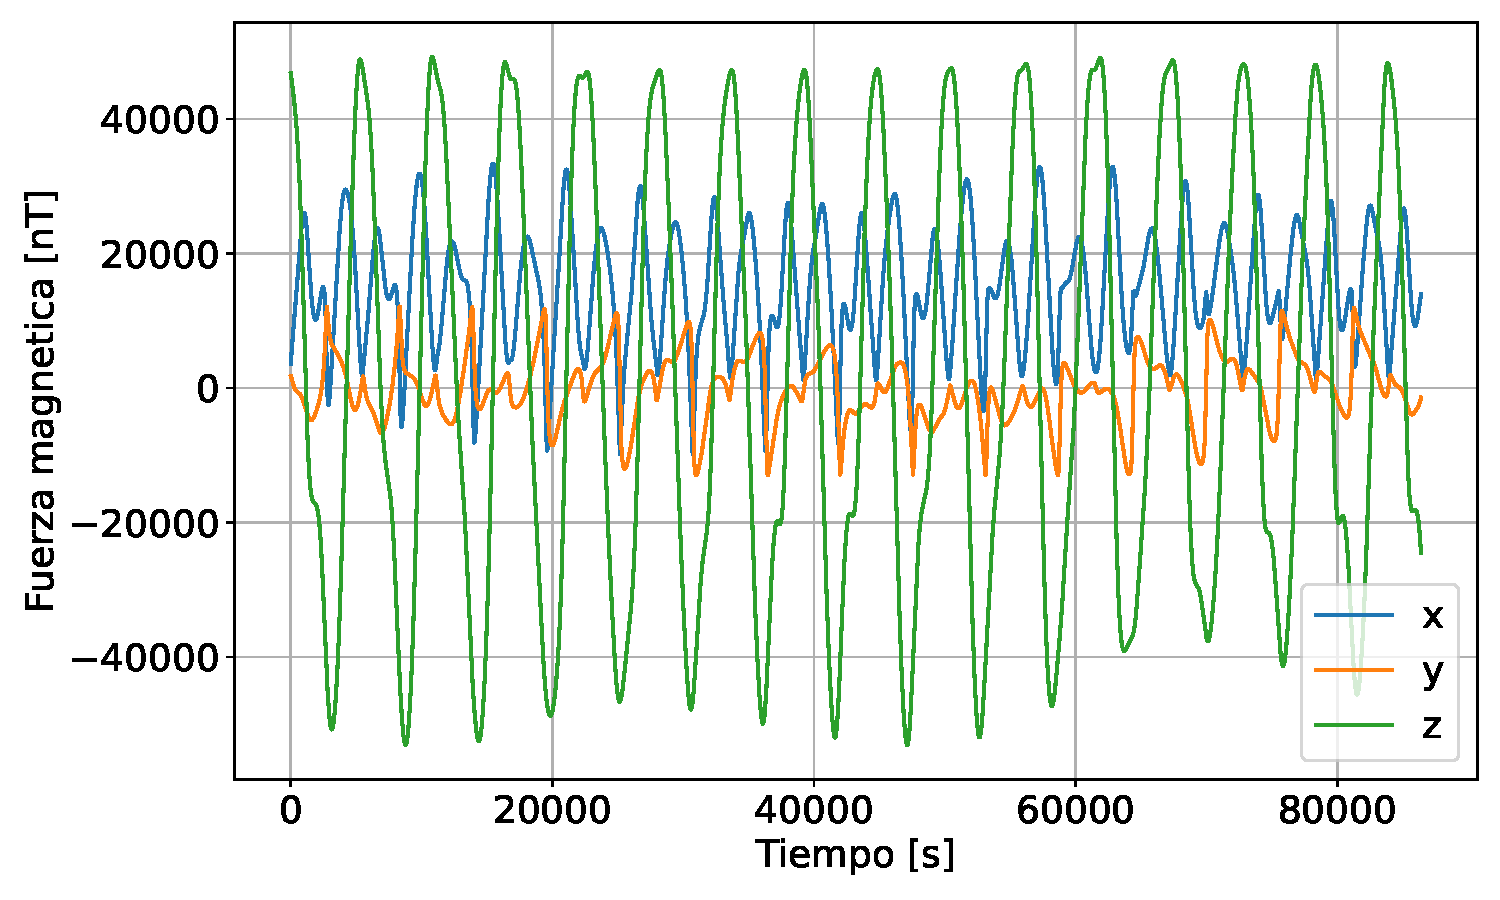
\includegraphics[width=0.65\textwidth]{bb.pdf}
	\caption{Componentes de las fuerzas magnéticas respecto a ECI que afectan al SUCHAI-3 con fecha inicial 01/11/2023 (Elaboración propia).}
	\label{fig:bb}
\end{figure}

\subsubsection{Cambios en los sistemas de referencia y vectores de observación}

Ya obtenidos los vectores sol y las fuerzas magnéticas en ECI, se aplica una matriz de rotación desde ECI a LVLH utilizando los vectores \gls{r} y \gls{v} calculados en la Sección 4.2 proveniente del SGP4. Dicha matriz de rotación se representa de la siguiente manera \cite{ref9}:

\[
	\vec{Z_O} = \frac{\vec{r}}{\|\vec{r}\|} \quad 	\vec{X_O} = \frac{\vec{v} \times \vec{Z_O}}{\|\vec{v} \times \vec{Z_O}\|} \quad 	\vec{Y_O} = \vec{Z_O} \times \vec{X_O} 
\]

\[
	R_{\text{ECI}}^O = 
	\begin{bmatrix}
		\vec{X_O}^T &
		\vec{Y_O}^T &
		\vec{Z_O}^T
	\end{bmatrix}
\]

Utilizando esta matriz, en conjunto con el cuaternión inicial estimado, el cual se representa como $R_{\text{ECI}}^{\text{body}}$, se obtiene la matriz de rotación que relaciona el marco de referencia del cuerpo con el orbital, mediante la siguiente relación:

\[
	R_O^{\text{body}} = (R_{\text{ECI}}^{O})^T \cdot R_{\text{ECI}}^{\text{body}}
\]

Mediante esta matriz de rotación, la cual puede ser transformada a un cuaternión $q_O^{\text{body}}$, se puede aplicar el control que será analizado en secciones posteriores utilizando una condición inicial en el sistema de referencia adecuado. Para la obtención de los vectores sol y las fuerzas magnéticas en el marco de referencia del cuerpo, se genera el cuaternión entre los marcos de referencia a medida que se estima en el siguiente paso de tiempo. Es relevante reconocer que se utilizan las mismas relaciones de rotación para la obtención de los vectores $B_O$ y $\vec{v}_{\text{sun}, O}$ usando los cuaterniones $q_{\text{ECI}}^{O}$.

\[
	(q_O^{\text{body}})^{-1} = [-q_0, -q_1, -q_2, q_3]
\]

\[
	B_{\text{body}} = (q_O^{\text{body}})^{-1} \cdot B_O \cdot q_O^{\text{body}}
\]

\[
	\vec{v}_{\text{sun, body}} = (q_O^{\text{body}})^{-1} \cdot \vec{v}_{\text{sun, O}} \cdot q_O^{\text{body}}
\]

\subsection{Algoritmos de estimación y control satelital}

Ya obtenidos los vectores de referencia y de observación, se puede estimar la orientación (cuaterniones) y la velocidad angular del satélite a través del tiempo. Para ello se estima la actitud actual mediante mediciones y métodos matemáticos, para posteriormente definir una acción de control que logrará apuntar hacia la actitud objetivo (sistema de referencia LVLH) utilizando un sistema de control automático.

\subsubsection{Conversión representación de rotación y \gls{EKF}}

Para la realizacion de la suite de simulación, se hace entrega de un cuaternión inicial tanto para el modelo que representa las mediciones llamada 'real' y otra condición inicial 'estimada' para cada paso del \gls{EKF}. Además, para el análisis de resultados, se utilizan los ángulos de Euler para una mayor comprensión conceptual y física de los cambios de orientación ocurridos en el satélite. En el Anexo \ref{ap:Z3} se presentan dichas conversiones matemáticas.

Se utilizó el \gls{EKF} de forma recursiva para estimar la actitud del satélite, tomando como referencia inicial el estado estimado. Este filtro fue implementado para su uso tanto con los magnetorquers como con las ruedas de reacción, utilizando modelos dinámicos lineales discretos. En cada caso, se ajustaron las matrices de estado A y de control B, mientras que la matriz de salida C se construyó a partir de las mediciones simuladas del magnetómetro y el sensor solar.

En cuanto a la matriz C, dado que depende de las mediciones del magnetómetro, las cuales varían con el tiempo, dicha matriz también cambia a lo largo de la simulación. Al intentar linealizar el control en la siguiente sección, las matrices A y B no varían con el tiempo, pero la matriz de salida sí, lo que dio origen al término "Semiextendido". Para más detalles sobre el diseño del filtro de Kalman "Semiextendido", se puede consultar el Anexo \ref{ap:Z4}.

\subsubsection{Controladores y actuadores}

Se ha optado por utilizar el controlador Proporcional-Derivativo (PD) debido a su simplicidad y a su capacidad para orientar el satélite hacia una posición específica. Adicionalmente, se ha simulado el controlador Linear Quadratic Regulator (LQR) para obtener una matriz de ganancia que garantice un control estable en ambos actuadores simulados. Sin embargo, es importante destacar que se logró un control estable únicamente con el controlador PD aplicado al magnetorquer; por lo tanto, el uso de este controlador se presenta solo para este actuador.

Para utilizar un controlador, es fundamental comprender la linealización del sistema, un proceso útil para simplificar modelos no lineales como las Ecuaciones~\ref{eq:cin_omega} y~\ref{eq:vect_dot} y facilitar el diseño de estrategias de control. Este proceso se basa en la aproximación de Taylor \cite{ref42}, que consiste en linealizar las ecuaciones alrededor de un punto de equilibrio.

Esto implica calcular las derivadas parciales de las funciones de estado con respecto a las variables de estado y de control. Las matrices resultantes, $A = \frac{\partial f(x,u)}{\partial x}$ y $B = \frac{\partial f(x,u)}{\partial u}$, representan la dinámica linealizada del sistema, generando así el modelo \gls{EE} mostrado a continuación.
\[
	\dot{x} = A x + B u
\]
Es importante destacar que la linealización proporciona una descripción local del comportamiento del sistema alrededor del punto de equilibrio, y por lo tanto, la validez de este enfoque depende de la proximidad del estado actual del sistema al punto de equilibrio.

Además, se optan por el magnetorquer\cite{ref14} y la rueda de reacción\cite{ref41} como actuadores, debido a la documentación encontrada sobre su utilización y su uso mayoritario en nanosatélites. Para conocer el álgebra y las consideraciones del diseño del control lineal a mayor detalle para cada actuador, se recomienda revisar el Anexo \ref{ap:Z5} y \ref{ap:Z6} respectivamente. 

\underline{Magnetorquer}

El punto de equilibrio para el caso del modelo dinamico con magnetorquer se muestra a continuación, cuyos valores representan que no existe diferencia de orientación entre los marcos de referencia del cuerpo y orbital, además de lograr que se minimice tanto la acción de control como la velocidad angular \cite{ref14}.

\[
	q_{\text{co}} = [0, 0, 0, 1] \quad	u = [0, 0, 0] \quad	\omega_{\text{co}} = [0, 0, 0]
\]



Los torques de control en sus tres componentes se representan en las Ecuaciones~\ref{eq:MT_x},~\ref{eq:MT_y} y~\ref{eq:MT_z}.


\begin{equation}
	\tau_{x,\text{mt}} = \left( \frac{b_x m_z - b_z m_x}{\|b\|} \right) b_z - \left( \frac{b_y m_x - b_x m_y}{\|b\|} \right) b_y
	\label{eq:MT_x}
\end{equation}

\begin{equation}
	\tau_{y,\text{mt}} = -\left( \frac{b_z m_y - b_y m_z}{\|b\|} \right) b_z + \left( \frac{b_y m_x - b_x m_y}{\|b\|} \right) b_x
	\label{eq:MT_y}
\end{equation}

\begin{equation}
	\tau_{z,\text{mt}} = \left( \frac{b_z m_y - b_y m_z}{\|b\|} \right) b_y - \left( \frac{b_x m_z - b_z m_x}{\|b\|} \right) b_x
	\label{eq:MT_z}
\end{equation}

Donde b son las fuerzas magnéticas en el marco de referencia del cuerpo y m es el momento dipolar del magnetorquer. Evaluando los valores deseados de $q_{\text{co}}$ y $\omega_{\text{co}}$ en las matrices $A$ y $B$ mencionadas en el Anexo \ref{ap:Z5}, se obtiene:

\[
	A = \begin{bmatrix}
		0 & 0 & 0 & 0.5 & 0 & 0 \\
		0 & 0 & 0 & 0 & 0.5 & 0 \\
		0 & 0 & 0 & 0 & 0 & 0.5 \\
		6\omega_{(0,o)}^2 [I_z - I_y] & 0 & 0 & 0 & 0 & 0 \\
		0 & 6\omega_{(0,o)}^2 [I_z - I_x] & 0 & 0 & 0 & \frac{\omega_{(0,o)} (I_x - I_y)}{I_z} - \omega_{(0,o)} \\
		0 & 0 & 0 & 0 & \frac{\omega_{(0,o)} (I_x - I_z)}{I_y} + \omega_{(0,o)} & 0
	\end{bmatrix}
\]

\[
	\bar{B} = \begin{bmatrix}
		0 & 0 & 0 \\
		0 & 0 & 0 \\
		0 & 0 & 0 \\
		\frac{-b_z^2 - b_y^2}{\|b\| I_x} & \frac{b_x b_y}{\|b\| I_y} & \frac{b_x b_z}{\|b\| I_z} \\
		\frac{b_x b_y}{\|b\| I_x} & \frac{-b_z^2 - b_x^2}{\|b\| I_y} & \frac{b_y b_z}{\|b\| I_z} \\
		\frac{b_x b_z}{\|b\| I_x} & \frac{b_y b_z}{\|b\| I_y} & \frac{-b_y^2 - b_x^2}{\|b\| I_z}
	\end{bmatrix}
\]

Debido a que aun cuando se implementa una linealización en el equilibrio, las fuerzas magnéticas de la Tierra siguen variando, se debe obtener una matriz de control representativa para su uso en el modelo espacio estado:

\[
	B = \frac{1}{T} \int_{t_0}^{t_{0+T}} \bar{B}(t) \, dt
\]

Para el caso del controlador LQR, con las matrices A y B y las matrices Q y R entregadas por el diseñador del control, se logra obtener la \gls{K} y ejercer el control en el modelo dinámico.

Por otro lado, para el controlador PD, se debe representar el modelo espacio estado de la siguiente manera:

\[
	\dot{x} = \hat{A} x
\]

Con: 

\[
	\hat{A} = A + BK
\]

\[
	K = \begin{bmatrix}
		K_{p,x} & 0 & 0 & K_{d,x} & 0 & 0 \\
		0 & K_{p,y} & 0 & 0 & K_{d,y} & 0 \\
		0 & 0 & K_{p,z} & 0 & 0 & K_{d,z} \\
		
	\end{bmatrix}
\]

Las constantes \(K_p\) y \(K_d\) son las constantes proporcionales y derivativas del controlador, y desempeñan un papel crucial en la determinación de la estabilidad del sistema. Estas constantes se ajustan de manera que los valores propios de la matriz \(A + BK\) sean negativos, lo que garantiza la estabilidad del sistema en lazo cerrado.

Los valores propios negativos son indicativos de que el sistema es asintóticamente estable, lo que significa que las respuestas transitorias del sistema convergen hacia el estado de equilibrio deseado sin oscilaciones ni divergencias. En otras palabras, los valores propios negativos aseguran que el sistema retorne a su estado de equilibrio después de cualquier perturbación, lo que es fundamental para el funcionamiento adecuado del sistema de control, con un rendimiento estable y robusto \cite{ref43}.
\\
\\
\\ 
\underline{Ruedas de reacción}

El punto de equilibrio para el caso del modelo dinamico con rueda de reacción se muestra a continuación, cuyos valores representan que no existe diferencia de orientación entre los marcos de referencia del cuerpo y orbital, además de lograr que se minimice tanto la acción de control como la velocidad angular del satélite y de cada rueda de reacción simulada (en este caso tres) \cite{ref41}.

\[
q_{\text{co}} = [0, 0, 0, 1] \quad u = [0, 0, 0] \quad 	\omega_{\text{co}} = [0, 0, 0] \quad 	\omega_{\text{rw}} = [0, 0, 0]
\]



Los torques de control son ejercidos por cada rueda de reacción de manera directa, siendo colocados en los tres ejes de referencia del marco de referencia del cuerpo del CubeSat por simplicidad. De esta manera, la rueda modelada en el eje x se representa mediante $\tau_{x, \text{rw}}$. Mismo caso para $\tau_{y, \text{rw}}$ y $\tau_{z, \text{rw}}$

Como se observa para los puntos de equilibrio, en este caso son nueves estados que se reemplazan en la matriz de estado A y B obtenida en el Anexo \ref{ap:Z6}, generando como resultado las siguientes matrices simplificadas:

\[
A_{11} = A_{13}
\begin{bmatrix}
	0 & 0 & 0 \\
	0 & 0 & 0 \\
	0 & 0 & 0 \\
\end{bmatrix} \quad
A_{12} = 
\begin{bmatrix}
	0.5 & 0 & 0 \\
	0 & 0.5 & 0 \\
	0 & 0 & 0.5 \\
\end{bmatrix}
\]

\[
A_{21} = 
\begin{bmatrix}
	 6 \omega_{0,o}^2 \left[I_z - I_y\right]  & 0 & 0 \\
	0 & 6 \omega_{0,o}^2 \left[I_z - I_x\right] + \frac{2 \omega_{0,o}^2 \left(J_x - J_z\right)}{J_y - I_{s1}}
	 & 0 \\
	0 & 0 &  -\frac{2 \omega_{0,o}^2 \left(J_x - J_y\right)}{J_z - I_{s2}}
	 \\
\end{bmatrix}
\]

\[
A_{31} = 
\begin{bmatrix}
	0  & 0 & 0 \\
	0 & - \frac{2 \omega_{0,o}^2 \left(J_x - J_z\right)}{J_y - I_{s1}}
	& 0 \\
	0 & 0 &  \frac{2 \omega_{0,o}^2 \left(J_x - J_y\right)}{J_z - I_{s2}}
	\\
\end{bmatrix}
\]

\[
A_{22} = -A_{32} = 
\begin{bmatrix}
	0  & 0 & 0 \\
	0  & 0 & \frac{\omega_{0,o} \left(J_x - J_z\right)}{J_y - I_{s1}} + \omega_{0,o} \\
	0 & \frac{\omega_{0,o} \left(J_x - J_y\right)}{J_z - I_{s2}} - \omega_{0,o} & 0	\\
\end{bmatrix}
\]

\[
A_{23} = -A_{33} = 
\begin{bmatrix}
	0 & 0 & 0 \\
	0 & 0 & -\frac{\omega_{0,o} I_{s2}}{J_y - I_{s1}}
	 \\
	0 & -\frac{\omega_{0,o} I_{s1}}{J_z - I_{s2}}
	 & 0 \\
\end{bmatrix}
\]

\[
A =
\begin{bmatrix}
	A_{11} & A_{12} & A_{13} \\
	A_{21} & A_{22} & A_{23} \\
	A_{31} & A_{32} & A_{33}
\end{bmatrix}
\]

\[
B =
\begin{bmatrix}
	0 & 0 & 0 \\
	0 & 0 & 0 \\
	0 & 0 & 0 \\
	\frac{1}{J_{x}-I_{s0}} & 0 & 0 \\
	0 & \frac{1}{J_{y}-I_{s1}} & 0 \\
	0 & 0 & \frac{1}{J_{z}-I_{s2}} \\
	\frac{1}{I_{s0}} - \frac{1}{J_{x}-I_{s0}} & 0 & 0 \\
	0 & \frac{1}{I_{s1}} - \frac{1}{J_{y}-I_{s1}} & 0 \\
	0 & 0 & \frac{1}{I_{s2}} - \frac{1}{J_{z}-I_{s2}} \\
\end{bmatrix}
\]

Una vez obtenidas las matrices A y B, dado que no hay vectores externos que varíen en el tiempo, como ocurre en el caso del magnetorquer, es posible utilizar un controlador LQR para guiar el sistema hacia el punto de equilibrio. Para ello, se debe diseñar el controlador seleccionando adecuadamente las matrices de ponderación Q y R, las cuales permiten ajustar el compromiso entre el rendimiento y el esfuerzo de control.

Es importante señalar que para ambos actuadores, la acción de control u se determina utilizando el vector de estado estimado, lo que permite aplicar torques realistas basados en las estimaciones obtenidas a través del \gls{EKF}. Además, el estado 'real' es aquel que simulará las mediciones de los sensores, mientras que el 'estimado' sera el que se utiliza en cada paso de tiempo del \gls{EKF}.

\subsection{Suite de simulación completa}

Ya tomadas las decisiones y generados los modelos dinámicos, se hace un resumen de las subsecciones mencionadas anteriormente:

\begin{itemize}
	\item \textbf{\textit{Uso del propagador SGP4 para la simulación de la dinámica orbital}}: Se eligió este debido a que presenta disponibilidad en el lenguaje de programación Python, además de ser de libre acceso y modela las perturbaciones necesarias en LEO a través del tiempo. Los demás propagadores como FreeFlyer y STK mencionados no son de libre acceso (tienen un alto costo monetario) y pueden no tener una conexión directa con las demás herramientas que se implementaran dentro del diseño del \gls{ADCS}.
	
	\item \textbf{\textit{Modelos orbitales y sensores por utilizar}}: En el caso de los modelos orbitales, se logra implementar los modelos de la fuerza geomagnética y del vector sol con éxito. Debido a ello, se simula el magnetómetro y el sensor de sol, debido a que se obtienen los vectores de observación a través de un cambio en el sistema de referencia de 'cuerpo' a 'orbital', además de la implementación del ruido característico del componente físico. Finalmente, el giroscopio aporta con la actualización del cambio angular en el CubeSat, obteniendo las velocidades angulares a través del tiempo.
	
	\item\textbf{\textit{Algoritmo de determinación de actitud seleccionado}}: Para la estimación inicial se elige un valor cercano a la condición inicial del modelo. Para obtener las estimaciones del estado a través del tiempo, se implementa el uso del metodo recursivo utilizando el \gls{EKF}.
	\\
	\\
	\item \textbf{\textit{Actuadores y controladores por utilizar}}: Se simularán magnetorquers y ruedas de reacción para el control de actitud en el simulador, ya que son los más comunes en nanosatélites. En ambos casos, se implementará el controlador Linear Quadratic Regulator (LQR), debido a su capacidad para ejercer un control estable sobre las matrices de estado A y de control 	B, utilizando matrices de ponderación Q y R adecuadamente diseñadas. Particularmente, para los magnetorquers también se utilizará un controlador Proporcional-Derivativo (PD) junto al LQR. Esto se debe a que la dinámica de actitud del satélite puede representarse mediante un cuaternión (componente proporcional) y la velocidad angular (componente derivativo), lo que es suficiente para orientar el satélite hacia una dirección deseada.
\end{itemize}

El esquema de la suite de simulación puede verse en la Figura~\ref{fig:suite}. En este diagrama, se muestra que el satélite primero debe determinar su posición y velocidad en la órbita. Para lograrlo, el propagador recibe parámetros de entrada como el TLE del satélite, una fecha de simulación y un tiempo de propagación. A continuación, el vector de posición se convierte a coordenadas \gls{GPS} para calcular la fuerza magnética, mientras que la fecha en formato JD2000, representada en el diagrama como t, se utiliza para determinar el vector solar. Ambos vectores, que están en el sistema de referencia ECI, se rotan al marco de referencia orbital utilizando los vectores de posición r y velocidad v, como se describe en la Sección xxx.

Por otro lado, el vector de estado estimado $x_{k}$ se utiliza tanto en el controlador como en el filtro de Kalman. En el controlador, se obtiene la matriz de ganancia K, lo que permite determinar la acción de control estimada, que luego es utilizada tanto en el modelo como en el filtro de Kalman.

En el diagrama, los bloques azules representan el flujo de control para las estimaciones, mientras que los bloques rojos corresponden a los vectores de estado reales para simular las mediciones. En ambos casos, los vectores magnético y solar se rotan al sistema de referencia del cuerpo (body frame) para generar las mediciones reales y estimadas del magnetómetro y el sensor solar. Estas mediciones se comparan dentro del filtro de Kalman para obtener el vector de salida. Con esto, se completa un paso de tiempo y el proceso continúa al siguiente.

\begin{figure}[H]
	\centering    
	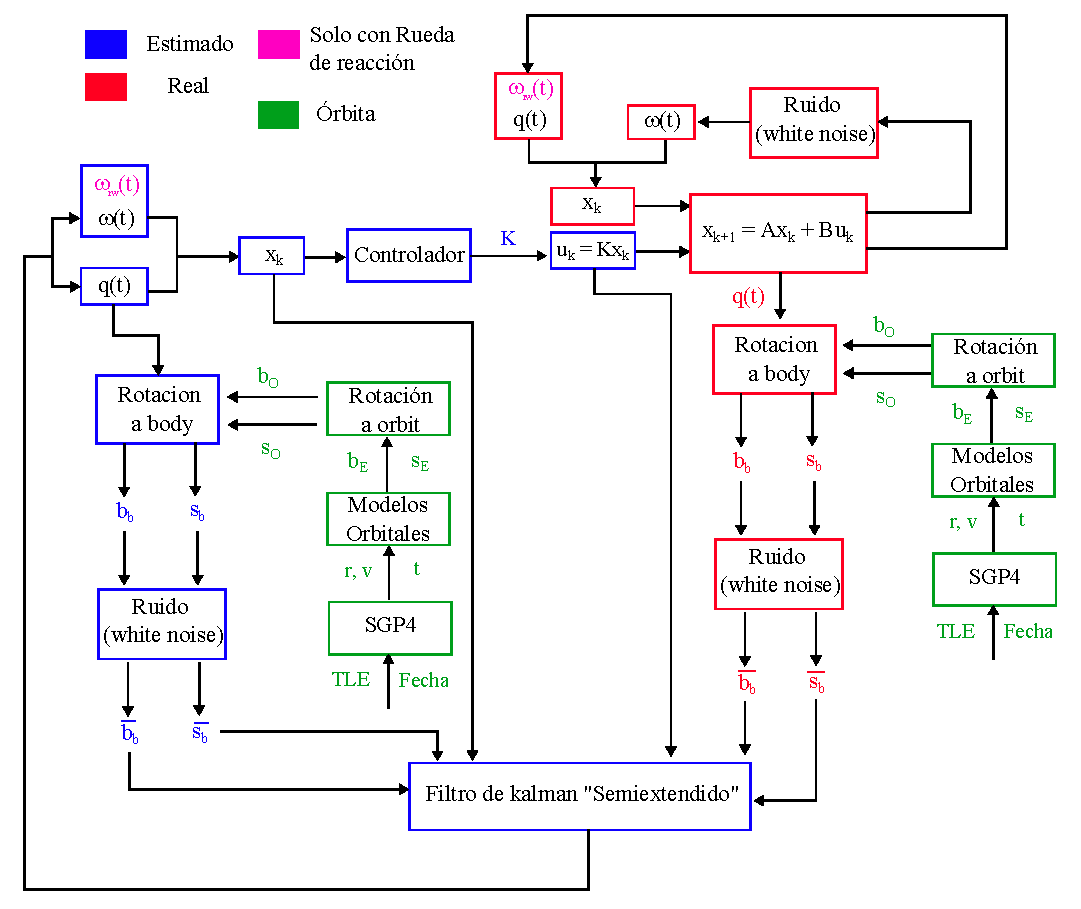
\includegraphics[width=0.9\textwidth]{suite.pdf}
	\caption{Diagrama de la suite de simulación completa (Elaboración propia).}
	\label{fig:suite}
\end{figure}